\documentclass[10pt,a4paper,hidelinks]{article}
\usepackage{lipsum}
\usepackage[bahasai]{babel}
\selectlanguage{bahasai}
\usepackage{url}
\usepackage{graphicx}
\usepackage[nochapters]{classicthesis} % nochapters

\begin{document}
    \pagestyle{plain}
    \title{\rmfamily\normalfont\spacedallcaps{Meningkatkan Efisiensi Pengolahan Limbah dengan proses yang berpusat pada Microbial Fuel Cell}}
    \author{\spacedlowsmallcaps{Eko J. Salim \& Gerraldo S. Candra}}
    \date{} % no date
    
    \maketitle
    
    \begin{abstract}
    	\noindent Proses pengolahan limbah sekarang meninggalkan banyak ruang untuk dikembangkan dan ditingkatkan. Limbah dapat menjadi sumber energi yang berharga --- sekitar 9 kali lebih banyak energi terkandung dalam limbah dibandingkan dengan energi yang diperlukan untuk mengolahnya dengan cara modern. Proses-proses yang tersedia sekerang jarang mempertimbangkan dan menggunakan hal ini, proses-proses ini juga sering tidak efisien dan 'kotor'.
Menggabungkan teknologi-teknologi pengolahan limbah menjadi sebuah proses yang berpusat pada Microbial Fuel Cell (MFC) dapat memecahkan masalah ini.
       % \noindent Current wastewater treatment processes and technologies left much to be desired. Wastewater could be a valuable source of energy --- about 9 times more energy are in wastewater compared to the energy needed to proccess them in a modern plant. Present processes do not generally take this into account moreover, they are also generally inefficient and 'unclean'. Combining present technologies, such as and especially Microbial Fuel Cell (MFC) could help alleviate these present issues considering wastewater treatment. 
    \end{abstract}
       
    \tableofcontents
    \section{Pendahuluan}
    \subsection{Latar Belakang}
    Proses pengolahan limbah yang ada sekarang tidak dapat memenuhi aspirasi masyarakat yang menginginkan air bersih, energi dan sumber daya dari limbah. Proses sekerang malah menggunakan energi yang signifikan. Konsumsi energi dari industri air diperkirakan adalah 2\% dari konsumsi listrik global. Penting sekali adanya proses pengolahan yang lebih efisien dalam konteks energi. Menurut Perserikatan Bangsa-Bangsa, diperkirakan tindakan mengingkatkan efisiensi adalah 65\% dari penghematan emisi global sampai dengan 2030.
    
    Dalam proses-proses yang menghemat energi ini, juga diharapkan kalau dapat diperoleh energi dan sumber daya dari limbah. Mengingat pentingnya mendaur ulang energi dan sumber daya untuk kelangsungan peradaban manusia sekarang ini, pendauran ulang dari limbah sangat diharapkan.
    
	\subsection{Identifikasi Masalah}
	\begin{itemize}
	\item Proses pengolahan limbah sekarang tidak dapat memenuhkan aspirasi masyarakat
	\item Dari proses pengolahan limbah, diharapkan energi, air bersih dan sumber daya
	\item Proses sekarang tidak hemat energi, 2\% dari total konsumsi listrik global adalah untuk air
	\item Penting didaur-ulangnya sumber daya dan energi dari limbah untuk memecahkan masalah energi dunia
	\end{itemize}
	\subsection{Batasan Masalah}
	Memperoleh air bersih, energi dan sumber daya dari limbah
	\subsection{Rumusan Masalah}
	Bagaimana cara  mendapatkan air, energi dan sumber daya dari limbah dengan cara efisien?
	\subsection{Tujuan Penelitian}
	\subsubsection{Tujuan Umum}
	Diperolehnya proses / rangkain proses yang sesuai untuk digunakan dengan Microbial Fuel Cell untuk memaksimalkan sepenuhnya ekstraksi (air bersih, energi, sumber daya, dan lain lain) dari limbah dengan efisien.
	\subsubsection{Tujuan Khusus}
	\begin{itemize}
	\item Mengidentifikasi kelemahan dan kelebihan dari proses-proses dan teknologi pengolahan limbah
	\item Meneliti kesesuaian Microbial Fuel Cell dengan proses-proses pengolahan limbah lainnya
	\item Memperoleh data penggunaan sistem Microbial Fuel Cell dengan berbagai tipe limbah
	\end{itemize}
	\subsection{Manfaat Penilitian}
	Dengan penelitian ini, diharapkan rangkaian proses yang sesuai dapat ditemukan dan mulai digunakan masyarakat untuk mengolah limbah. Jika digunakan, masyarakat dapat menjadi lebih hijau dan berdikari.
	\section{Tinjauan Pustaka}
    \subsection{Kajian Teori}
    Banyak teknologi dapat digunakan untuk pengolahan limbah: dari sistem  \textit{activated sludge} sampai \textit{vacuum evaporation}. Menggabungkan teknologi-teknologi yang ada ini menjadi sistem yang berpusat pada Microbial Fuel Cell dapat menghasilkan pengolahan limbah yang berkelanjutan.
    %Various technologies are available for wastewater treatment: from activated sludges to vacuum evaporation. Combining these technologies below could lead into a sustainable wastewater treatment especially in a MFC-centered treatment process.
    \subsubsection{Microbial Fuel Cell}
    Microbial Fuel Cell adalah alat yang menghasilkan arus menggunakan bakteri. bakteri di dalam MFC bekerja sebagai sebuah katalis untuk mengoksidasi zat organik maupun zat anorganik. Elektron hasil dari oksidasi ini bergerak menuju elektroda dan akhirnya menuju katoda dari anoda. Bagaimana cara elektron ditransfer ke anoda adalah perbedaan antara MFC dengan penengah dan tanpa penengah. Di MFC dengan penengah, ada penengah redox yang mengangkut elektron ke anoda. Jika tidak ditambah mediator eksogen, MFC tersebut dikatakan sebagai MFC tanpa penengah. Dalam MFC tanpa penegah, transfer elektron bisa dilakukan dengan cara: \textit{direct membrane associated electron transfer}, \textit{bacteria's nanowire}, dll. 
    %Microbial fuel cells are devices that drives a current using bacterias. Bacterias in a microbial fuel cell serve as catalyst to oxidize both organic and inorganic matters.  The electrons from this oxidation are transferred to the anode and then to the cathode.  The 'how' electrons are transferred to anode serves as the distinction between two general types of MFC. In mediator microbial fuel cell, there exists a redox mediator which ‘shuttles’ electrons to the anode. A microbial fuel cell is classified as a mediator-less MFC if no exogenous mediators are added,  the method ofelectrons transfer in these instances can be by the following: direct membrane associated electron transfer, bacteria’s ‘nanowires’ . . .


Di hampir semua MFC, elektron yang mencapai katoda bergabung dengan proton yang membaur dari anoda dna juga dengan oksigen dari udara; produk hasil penggabungan ini adalah air. Oksidator kimia juga dapat digunakan.
%In most MFCs, the electrons that reach the cathode combine with protonsthat diffuse from the anode and oxygen provided from the  air;  the  resulting  product  is  water.   Chemical  oxidizers  may  also  be used however because they need to replaced, they are not practical outisde laboratory use.


Karena MFC 'memakan' zat organik dan anorganik dan juga memproduksi listrik, MFC dapat digunakan dalam pengolahan limbah. Banyak riset telah meneliti tentang MFC dan pengolahan limbah, dari efektivitasnya dalam mengolah limbah intensitas tinggi sampai menambahkan efektivitas MFC dengan \textit{spiral spacer}.
%As MFCs break down organic matters and produce electricity, MFCs have found a use in wastewater treatment.


Dalam proses pengolahan berbasis MFC, kelemahan dan kelebihan MFC  harus dipertimbangkan. MFC yang sekarang kurang cocok dalam mengolah limbah intensitas tinggi. Isu \textit{scaling} juga adalah sebuah kelemahan MFC. Dengan menggabungkan teknologi MFC dengan teknologi lain, kita dapat mengatasi kelemahan-kelemahan dari MFC.
%In MFC-centered treatment process, weaknesses and advantages of MFC must be considered. MFC technologies fall short in treating high-intensity wastewater/sludge and scaling. However, numerous researches have proposed many and various solutions to MFC's shortcoming. 
	\begin{figure}[!ht]
	\centering
		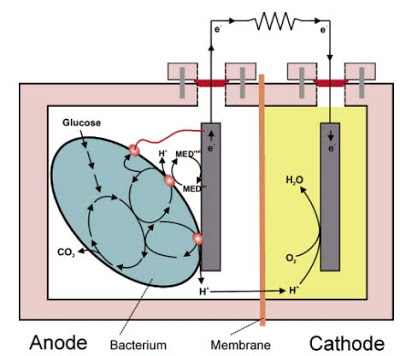
\includegraphics[scale=0.75]{gfx/mfc}
		\caption{Microbial Fuel Cell}
	\end{figure}
    \subsubsection{Anaerobic Digestion}
    Anaerobic digestion atau pencernaan anaerobik adalah proses dimana bakteri memecah zat \textit{biodegradable} saat tidak adanya oksigen. Pencernaan anaerobik dapat menghasilkan metana. Proses ini dimulai dengan hidrolisis oleh bakteri, polimer organik bersifat tidak larut diolah untuk digunakan bakteri lain. Bakteri \textit{acidogenic} mengubah gula dan asam amino menjadi asam asetat dan juga ammonia, hidrogen dan karbon dioksida. Kemudian, produk ini diubah menjadi metana dan karbon dioksida. Metana yang dihasilkan ini dapat digunakan untuk menghasilkan listrik.
    
Pecernaan anaerobik sudah dibuktikan dapat mengolah limbah intensitas tinggi, salah satu kelemahan dari MFC. Dari pengolahan limbah intensitas tinggi, hasilnya dapat digunakan oleh MFC untuk menghasilkan listrik dan lebih membersihkannya.
    \subsubsection{Microalgae treatment}
    Microalgae atau mikroalga dapat menjadi proses olahan setelah proses MFC. Mikroalga dapat mengolah nutrisi dan logam berat. Hasil olahan adalah biomassa yang dapat digunakan untuk produksi listrik.
    
	\begin{figure}[!ht]
	  \centering
		  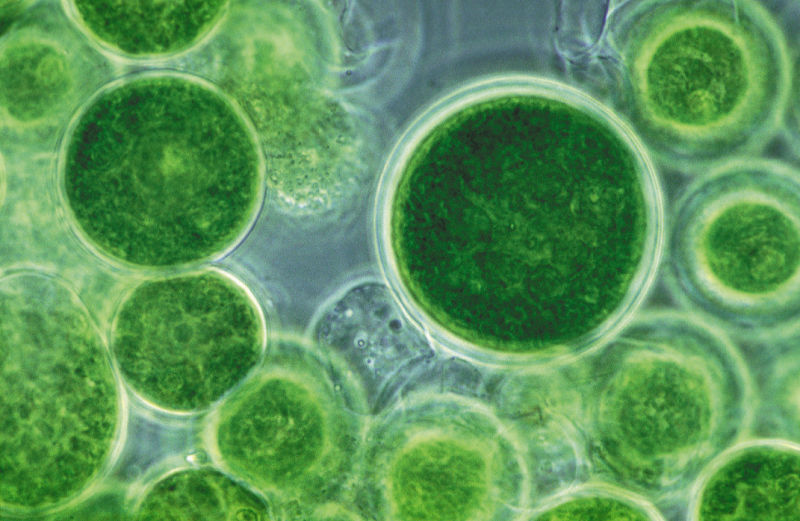
\includegraphics[width=0.75\textwidth]{gfx/microalgae}
	  \caption{Mikroalga}
	\end{figure}

    \subsubsection{Membrane Seperation}
    \subsubsection{Struvite Precipitation}
    \subsection{Hipotesis}
    \section{A Section}
    \lipsum[1]
    
    % Bibliography
    \nocite{*}
    \addtocontents{toc}{\protect\vspace{\beforebibskip}}
    \addcontentsline{toc}{section}{\refname}    
    \bibliographystyle{plain}
    \bibliography{Bibliography}
\end{document}